\chapter{Analysis}\label{ch:analysis}

\summary{
We have now devised a fully-fledged document layout system that works across many platforms. In this chapter we analyse the system both quantitatively and qualitatively to answer the question, ``is it any good?''
}

%\section{View-time Operations}

\section{Quantitative}

Chapter~\ref{ch:intro} (and in particular Section~\ref{sec:goodtypesetting}) provides an overview of some of the operations required when laying out a document. This chapter goes into a little more detail, and contrasts the operations required to view fixed and flowable documents against the operations required to view malleable documents.

\subsection{Fixed Document Formats}
Documents in a fixed format are rendered in a manner similar to the following:
{\singlespacing
\begin{lstlisting}
parse and tokenise the document layout instructions;
foreach (layout instruction) {
    interpret and execute the instruction;
}
paint the results to the screen;
\end{lstlisting}
}
Crucially, the layout instructions are declarative, and do not permit computation, which ensures that the document is always rendered identically.\hspace{0pt}\cite{Bagley2007}

\newpage
\subsection{Flowable Document Formats}

When a document in a flowable format is to be laid out, the process is as follows:
{\singlespacing
\begin{lstlisting}
parse the source to identify flowable blocks;
foreach (flowable block) {
    apply a line-breaking algorithm;
}
paint the results to the screen;
\end{lstlisting}
}

This process generates information similar to that contained in fixed-format documents, which is then used to drive the painting of contents to the screen.

The line breaking algorithm can be as simple as or complex as desired. In most cases, the line-breaking algorithm used by flowable documents is reasonably simple, and will take a first fit approach. This will be of the form:

{\singlespacing
\begin{lstlisting}
parse block to identify all possible breakpoints;
while (non-breakable items remain to be laid out) {
    place one item on the current line;
    if (there is not space for the next item) {
        adjust spacing between items to justify;
        move to a new line;
    }
}
\end{lstlisting}
}

As is noted in Section~\ref{sec:goodtypesetting}, first-fit algorithms do not generally result in well-typeset output. The simplest of these algorithms will not attempt to identify potential hyphenation points. More complex layout algorithms that search for ``optimal'' layouts usually require a considerable amount of backtracking.

\newpage
\subsection{Malleable Documents}

The layout algorithm for a malleable document is as follows. First, the penalties are calculated:

{\singlespacing
\begin{lstlisting}
foreach (included galley rendering) {
    compute penalty for the rendering at current page width;
}
select the rendering with the minimum penalty;
\end{lstlisting}
}


Then, using the galley rendering that has the lowest penalty, the content is laid out onto the screen:

{\singlespacing
\begin{lstlisting}
foreach (paragraph-level item in selected galley rendering){
    foreach (line-level item in paragraph) {
        use precomputed data to place words;
    }
}
paint the results to the screen;
\end{lstlisting}
}
Crucially, a number of complex steps have been moved from view-time to compile-time (as they are for fixed-format documents) but without flowability being sacrificed:
\begin{itemize}
 \item The source is already parsed into a form optimised for layout
 \item The line-breaking algorithm has been entirely precomputed
\end{itemize}
One step has been added: each included galley rendering must be examined once before layout, in order to ascertain its ``penalty'' for use. The penalty is based entirely on the width of the page, and the \gls{measure} (width) of the galley rendering.%, and is described in more detail in Section~\ref{sec:layout}.

This penalty is calculated by taking the extra required horizontal whitespace (which can be envisaged as slack between columns) and weighting this to further penalise large numbers of columns. This weighting is achieved by multiplying by a smaller-than-linear function of the number of columns, such as a square root or logarithm.

Many low-power processors do not come with floating-point hardware as standard (for example the \textsc{arm} range of processors) which might suggest that these are poor choices of functions since they must be emulated using integer and bitwise operations only. This is not particularly important, for a number of reasons. Firstly, it has been shown previously\hspace{0pt}\cite{Lomont2003} that it is often possible to use mathematical analysis to find extremely good approximations for such functions. Secondly, the range of inputs to such a function would be limited to integers ranging from 1 to (in an extreme case) about 20, so the values could be pre-computed and stored in a lookup table. Thirdly, the penalty (and hence the root or logarithm) is calculated precisely once for each included galley rendering: in section~\ref{sec:inc-renderings} it is suggested that between three and seven galley renderings should be included in any one document. Given these facts, it is clear that there should be little impact from using such a function in the penalty calculation.

\vspace{2em}

Most importantly, since the line-breaking algorithm has been moved to compile-time, there is no longer any requirement to limit its complexity. In fact, should the need (or desire) arise, the text layout can be hand-tuned, or \emph{entirely hand-typeset}, with no consequences at view-time.


\subsection{Handling of Floats}

The grid-based layout system devised in Section~\ref{sec:gridlayout} works in a similar manner to a first-fit line-breaking algorithm, in that it places elements on the page in order, in the first place they will fit. In the case of this system, each element is a floatable figure or line of text. Elements that are the same size as a single grid cell, such as lines of text set in the main point size, can simply be placed in the first empty slot in the current column, or the first empty slot in the next column, should there be no empty spaces.  For the placement of elements that are larger than a single grid cell, there is some overhead required to step through the grid until a suitable position can be found. Once a position has been found, each grid cell that it overlaps must be marked as being reserved.

In the worst case, this algorithm does have a greater-than-linear time complexity. In practice, so long as the number of floats does not become excessive (which would cause the grid to be walked many times to search for suitably large gaps) the algorithm runs in linear time.

The placement of floats is subject to certain constraints: they must span integer multiples of columns, and can only be placed aligned to grid cells. This is very different to the model used for floats in \gls{html}, whereby floats may be positioned arbitrarily, and text flowed around them. Although a little more restrictive than \gls{html}, this system is capable of producing layouts that lend themselves to many types of document that are likely to be read on \ebook{} readers. The next chapter discusses this in more detail.


\section{Qualitative}
\label{sec:aesthetics}

\subsection{Placement of Floats}
Since all text layout is precomputed, the only remaining concern is that the columns of text and floats are laid out in a pleasing manner. Plass\hspace{0pt}\cite{Plass1981} devised a system to perform optimal placement of floats within text, whereby float placement is penalised by the square of the distance from its intended position. He showed that this problem was NP-hard, but he also showed that a similar (but less ``optimal'') system using linear penalties could be made computationally tractable.

Br\"uggemann-Klein et al.\hspace{0pt}\cite{Bruggemann-Klein1995} suggested that Plass's method is only optimal for a given definition of ``optimal''. They proposed that a superior metric for float placement is to minimise the number of page turns that a reader must perform when reading the document from front to back. This is a desirable characteristic for a pagination algorithm that runs on an \ebook{} reader, because page turns tend to be slow, particularly on devices with electronic paper displays. Unfortunately, the algorithm used runs in quadratic time, which limits its usefulness to this system.

In essence, the assumption that Plass's float placement algorithm produces the most optimal layouts may be slightly short-sighted: \emph{other pagination schemes are available!} Clearly, using a computationally intractable algorithm such as Plass's will have significant impact on the demand for computation at view-time. As with many facets of the system described in this thesis, the float placement algorithm was chosen with efficiency in mind.

The float placement algorithm that has been developed for use with the malleable document system also attempts to minimise the distance between the actual and intended positioning of floats: if a float can be placed directly at its intended position, then it will be, otherwise it will be placed in the next available space. (Figure~\ref{fig:gridlayout} on page~\pageref{fig:gridlayout} demonstrates this process.)

Whilst this algorithm does not perform any lookahead or backtracking in order to place floats optimally, experiments have shown that in most cases, floats are placed directly in their intended positions or at the top of adjacent columns, and are only occasionally moved across page boundaries. Figures \ref{fig:example-portrait}, \ref{fig:example-landscape}, and~\ref{fig:example-ereader} show some examples of layouts produced using this algorithm, and Figures \ref{fig:example-latex} and~\ref{fig:example-html} show some comparative renderings of the same document, produced by \LaTeX{} and a web browser respectively. The output of the malleable document system looks very similar to that of \LaTeX, and very different from that of the web browser.

As it stands, the algorithm does not avoid widowed or orphaned lines, nor single lines directly before or after floats. This can be seen clearly in Figure~\ref{fig:example-ereader} at the top of the fourth page, where the float has spanned both columns and taken up all the space on the page, with the exception of one line at the top of each column. It would not be too difficult to add a constraint that states that single lines of text at the top or bottom of the page should never be allowed, which could be enforced by leaving extra lines blank, pushing the text forward, though it is possible that this may harm the balance of the page if it causes columns to have uneven lengths.

\todo{link to appendix for sample layouts}

\subsection{Measures of Aesthetic Quality}
In their 2004 paper, Harrington et al.\hspace{0pt}\cite{Harrington2004} identified nine aesthetic measures for automated document layout. A number of these measures (alignment, regularity, uniform separation, white-space free-flow, uniformity) are inherently well satisfied by this system, due to its use of a grid to provide regular layout. 

\subsection{User Study}

In order to establish the most appropriate range of galleys to include in a malleable document, as discussed in Section~\ref{sec:inc-renderings}, a user study was conducted. This was also used as a chance to get some general feedback about the malleable document system from a wide range of real-world users.

\todo{the following}

* state rationale, number of respondents etc (overview)

* state questions \& intentions from them

* state method of comparing different variants

* state reasoning behind choice of renderings (cite chapter 2)

* Mention extra data recorded

* Pick some decent comments

* Pick some interesting stats from tScreenSize

Please rate the following statements based on how closely you agree or disagree with them.

For each, choose a number from 0 to 10, where 0 is "I strongly disagree", 5 is neutral, and 10 is "I strongly agree".
\begin{itemize}
\item The document layouts produced were well-adapted to fit my screen.
\item I could adequately customise the document layout to suit my personal reading preferences.
\item I would preferentially choose a document layout system like this to read long text-based web pages.
\item I would preferentially choose a document layout system like this to read PDFs.
\item I would preferentially choose a document layout system like this to read ebooks.
\end{itemize}


\begin{table}
  \footnotesize
  \myfloatalign
  \begin{tabular}{ccccccccccc}
    \toprule
    rendering id & range & step & n & respondents & q1 & q2 & q3 & q4 & q5 \\
    \midrule
    A & $2-3$ & $1$   & $3$  & $9$ & $6.8$ & $6.3$ & $5.7$ & $7.1$ & $6.8$ \\
    B & $2-4$ & $1$   & $4$  & $6$ & $7.7$ & $6.7$ & $6.0$ & $6.3$ & $5.8$ \\
    C & $2-6$ & $1$   & $6$  & $8$ & $7.1$ & $6.6$ & $4.5$ & $6.0$ & $5.8$ \\
    D & $2-4$ & $0.5$ & $6$  & $7$ & $8.1$ & $7.7$ & $5.9$ & $5.9$ & $7.4$ \\
    E & $2-6$ & $0.5$ & $10$ & $5$ & $8.6$ & $8.0$ & $8.6$ & $8.0$ & $8.4$ \\
    F & $2-6$ & $2$   & $4$  & $6$ & $6.5$ & $7.2$ & $5.3$ & $7.0$ & $8.0$ \\
    \bottomrule
\end{tabular}
  \caption[Short Caption]{Long Caption}
  \label{tab:studyavgs}
\end{table}

\begin{sidewaysfigure}
  \begin{center}
  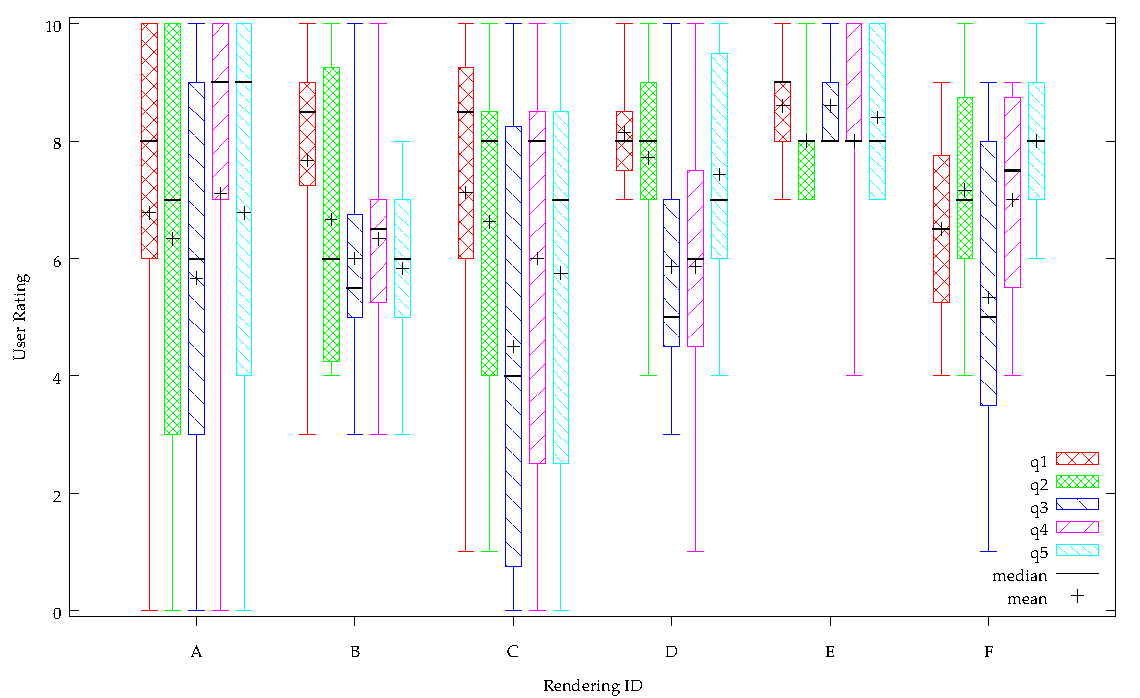
\includegraphics[height=0.5\textheight]{gnuplot/survey.pdf}
  \end{center}
  \caption[Short Caption]{Loooooooong caption}
  \label{fig:survey}
\end{sidewaysfigure}



%   - Greeking\\
%       - Default browser layout vs mine\\
%       - Look at \cite{Harrington2004} for some measures and say why mine is awesome\\
%   - some discussion of choices of galley widths for best performance


\section{Summary}
The malleable document system devised in this thesis was designed to be used for linear documents whose content is primarily text. Examples of such documents would be novels and scientific papers, but not reference books or graphic-heavy documents such as comics or children's picture books.

The layouts produced by this system are visually very similar to those of both newspapers and scientific papers, and can be flowed to fit virtually any page size. For smaller screen sizes, where single- or double-column spreads occur, the layouts closely resemble those of physical books and magazines.

%\todo{Sum up a bit better}
